\section{Background and Related Work}
\label{sec:problem}

In this section, we first introduce several common neural networks model,
Logistic Regression (single neuron) model, Multi-Layer Perceptron (MLP) model,
and Convolutional Neural Network (LeNet) model. Then we summarize and compare
our work to several related works that introduce noise into those models to
improve accuracy.

\subsection{Neural Network Models Explained}

The simplest form of a neural network, which is also the primary component of
any neural network model, is a single neuron. Figure~\ref{fig:lr-diag} illustrates a
single-neuron neural network, which is also known as the Logistic Regression
(LR) model. The neuron shown in the figure consumes a vector of numbers (X) as
inputs, and produces a single number as its output, which typically represents
the prediction result by the model. The neuron stores a vector of weights (W),
with each weight represents how positively or negatively each input affects the
output. The output of the neuron and the update to the neuron's weight can be
computed as follows:
\[
  Output = \tanh(W \cdot X)
\]
\[
  W_{new} = W_{old} - learningRate \cdot \nabla_{W_{old}} \cost(W)
\]

A Multi-Layer Perceptron (MLP) model is essentially multiple layers of neurons
connected by a network. Figure~\ref{fig:mlp-diag} illustrates a simple example of
such model, which is composed of three layers. The first layer is the input
layer, which provides the raw inputs to the next layer. The second layer is the
hidden layer, whose input is fully connected to the input layer, and output
fully connected to the output layer. The hidden layer is known to be capable of
extracting features from the input. The third layer is the output layer, which
outputs the prediction results for the data. Note that the figure shows only an
example of such model, the model can become ``deeper'' to extract more implicit
features from the raw input if we add more hidden layers between input and
output layers, which are fully connected to the layers next to each other.

\begin{figure}[!h]
\centering
\begin{subfigure}{.49\linewidth}
  \centering
  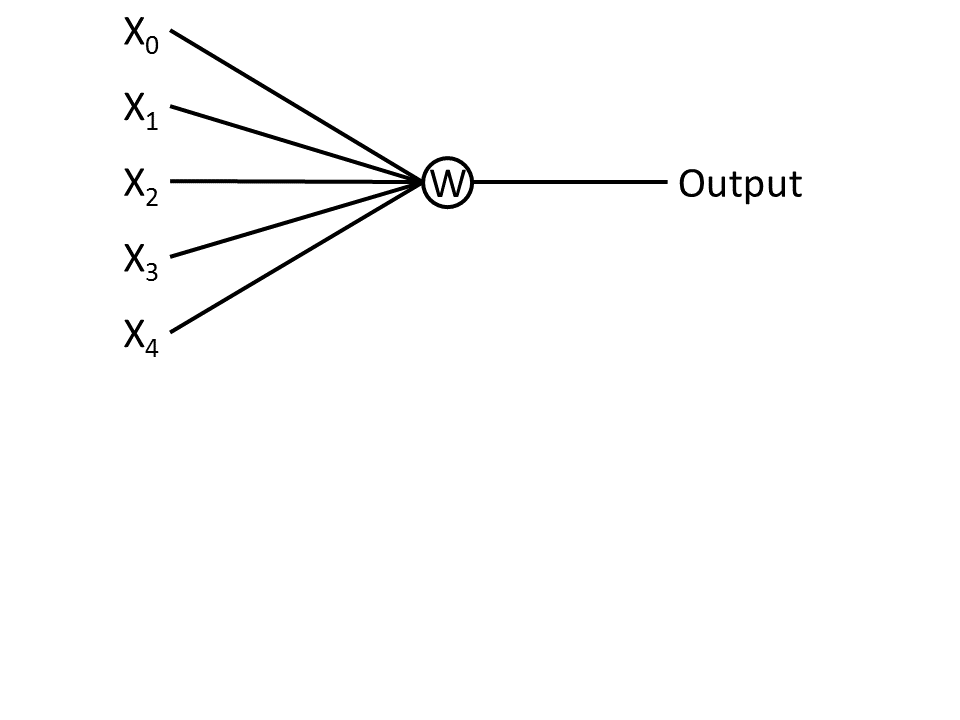
\includegraphics[trim=0 260 0 0,clip,width=\linewidth]{f-figs/lr-diag}
  \caption{Single-layer neural network (LR) model.}
  \label{fig:lr-diag}
\end{subfigure}
\begin{subfigure}{.5\linewidth}
  \centering
  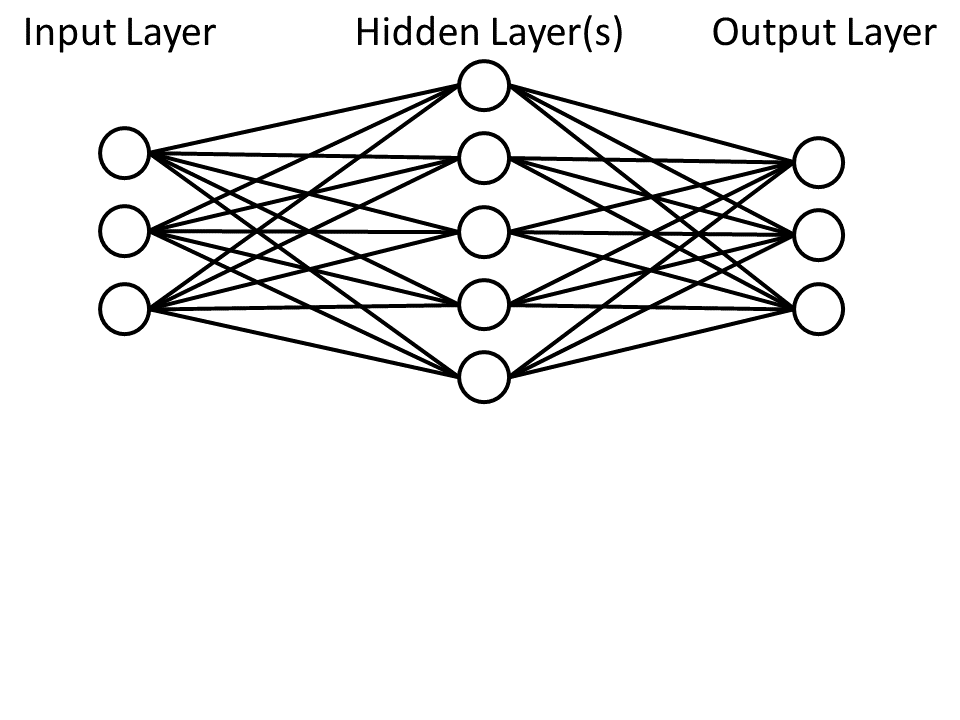
\includegraphics[trim=0 230 0 0,clip,width=\linewidth]{f-figs/mlp-diag}
  \caption{Multi-Layer Perceptron (MLP) model.}
  \label{fig:mlp-diag}
\end{subfigure}
\caption{Illustration of two neural network models.}
\end{figure}

A Convolutional Neural Network (LeNet) model adds multiple convolution layers in
addition to the MLP model. Figure~\ref{fig:lenet-diag} illustrates an example of this
model. In the convolution layer, multiple steps are processed. First, the input
is transformed into a two-dimensional array. Then a sliding window which
contains a small two-dimensional weight vector is applied to the input. The
sliding window is capable of extracting 2-D features from the inputs such as
images. Finally, the processed input is downsampled by a 2x2 matrix, which
reduces the size of the input by 4. In this figure, we show an example which
contains two convolution layer and a hidden layer. We can also have a more
complex model by adding more convolution layers or more hidden layers, which
also allows the model to extract more implicit features.

\begin{figure}[!h]
\centering
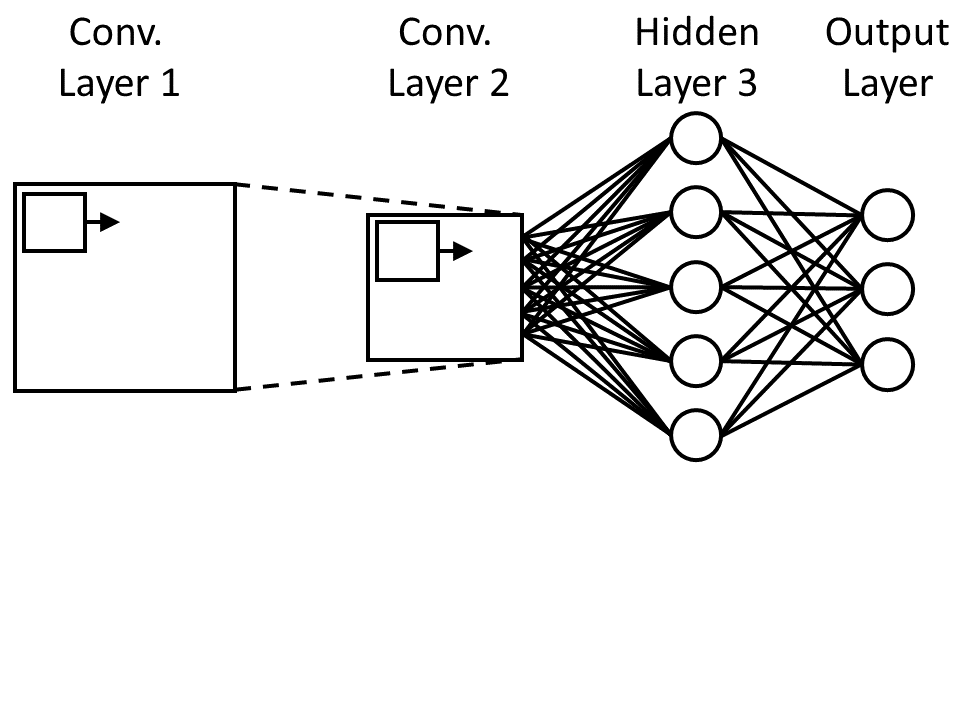
\includegraphics[trim=0 190 0 0,clip,width=0.6\linewidth]{f-figs/lenet-diag}
\caption{Convolutional Neural Network (LeNet) model.}
\label{fig:lenet-diag}
\end{figure}

\subsection{Comparison with Related Works}

We summarize three recent works that explain and explore three mechanisms to
introduce noise into a multi-layer neural network (mlp). Dropout proposes to
regularize fully connected neural networks by probabilistically dropping an
output (set to zero) of a hidden layer neuron~\cite{hinton2012improving} (i.e.,
with a low probability $(1-p)$, one of the output of a hidden layer neutron is
set to $0$ in the forward propagation process).  This can effectively decrease
test error rates by preventing over-fitting of the model. Inspired by
Dropout~\cite{hinton2012improving}, DropConnect proposes to probabilistically
drop a weight of a hidden layer neuron (as opposed to an output of a hidden
layer neuron in DropConnect)~\cite{wan2013dropconnect}. Maxout extends Dropout
and DropConnect by probabilistically set an output or a weight of a hidden layer
neuron to maximum value~\cite{goodfellow13maxout}. While these works attempts to
explore similar ideas as our work, we believe our work is much more
comprehensive than these works as we systematically and experimentally explored
various noise models, various noise locations, and various neural networks.



